\documentclass[biblatex]{mooiman_memo}
\addbibresource{./ref.bib}

\newcommand{\ii}{{\rm i}}
\newcommand{\Dx}{\Delta x}
\newcommand{\Dy}{\Delta y}
\newcommand{\Dt}{\Delta t}
\renewcommand{\vec}[1]{\mbox{\boldmath $#1$} }
\newcommand{\mat}[1]{\mbox{\boldmath ${\rm #1}$} }
\newcommand{\half}{\frac{1}{2}}
\newcommand{\quart}{\frac{1}{4}}
\newcommand{\abs}[1]{\left| #1 \right|}
\newcommand{\Sabs}{\textsl{Sabs}\xspace}
\newcommand{\eps}{\varepsilon}

\newcommand{\rhsadv}{{\it rhs}_{\it adv}}
\newcommand{\rhsmom}{{\it rhs}_{\it mom}}
\newcommand{\rhscont}{{\it rhs}_{\it cont}}
\newcommand{\GRADc}{{\it \widehat{GRAD}}_{\it c}}
\newcommand{\GRADu}{{\it \widehat{GRAD}}_{\it u}}
\newcommand{\GRADh}{{\it \widehat{GRAD}}_{\it h}}

\newcommand{\deltares}{Deltares\xspace}
\newcommand{\maplemath}{\textbf{Some MapleSoft math}}

\begin{document}
    \memoTo{to whom it may concern}
    \memoConfidentialUntil{}
    \memoDate{\today~\currenttime}
    \memoVersion{001}
    \memoFrom{Jan Mooiman}
    \memoTelephone{+31\,(0)6\,4691\,4571}
    \memoEmail{jan.mooiman@deltares.nl}
    \memoSubject{Atmospheric chemistry}
    \memoCopy{}

    \mooimantitle
    %------------------------------------------------------------------------------

\section{Atmospheric chemistry}
Example taken from \cite[eq.\ 1.1, page 7]{HundsdorferAndVerwer2003}.

We illustrate the mass action law by the following three reactions between oxygen $O_2$, atomic oxygen $O$, nitrogen oxide $NO$, and nitrogen dioxide $NO_2$:
\begin{align}
    NO_2 + h\nu & \xrightarrow{k_1} NO + O, \\
    O + O_2 & \xrightarrow{k_2} O_3, \\
    NO + O_3 & \xrightarrow{k_3} O_2 + NO_2.
\end{align}
The corresponding ODE system reads
\begin{align}
    \pdiff{u_1}{t} & = k_1 u_3 -k_2 u_1
    \\
    \pdiff{u_2}{t} & = k_1 u_3 - k_3 u_2 u_4 +\sigma_2
    \\
    \pdiff{u_3}{t} & = k_3 u_2 u_4 - k_1 u_3
    \\
    \pdiff{u_4}{t} & = k_2 u_1 - k_3 u_2 u_4
\end{align}
with $\vec{u}(0) = (0.0, \num{2.0e-1}, \num{2.0e-3}, \num{2.0e-1})^T$ and $\sigma_2 = \num{e-7}$, and the coefficients $k$ are defined as (the given conditions for are different from the  conditions as defined in \cite[page  8]{HundsdorferAndVerwer2003}):
\begin{align}
    k_1 & = \begin{cases}
        10^{-5} \exp{(7\ {\it g}(t))}
        \\
        \num{e-40}, \qquad \text{during  night}
        \end{cases}
        \\
        k_2 & = \num{2.0e-2}
        \\
        k_3 & = \num{1.0e-3}
\end{align}
with
\begin{align}
    {\it g}(t) =\left(\sin\left(\frac{\pi}{16} (t_h - 4)\right)\right)^{0.2}, \qquad t_h = \frac{t}{3600};
\end{align}
where $t_h$ is the time in hours.

Some results are:
\begin{figure}[H]
    \begin{subfigure}{0.5\textwidth}
        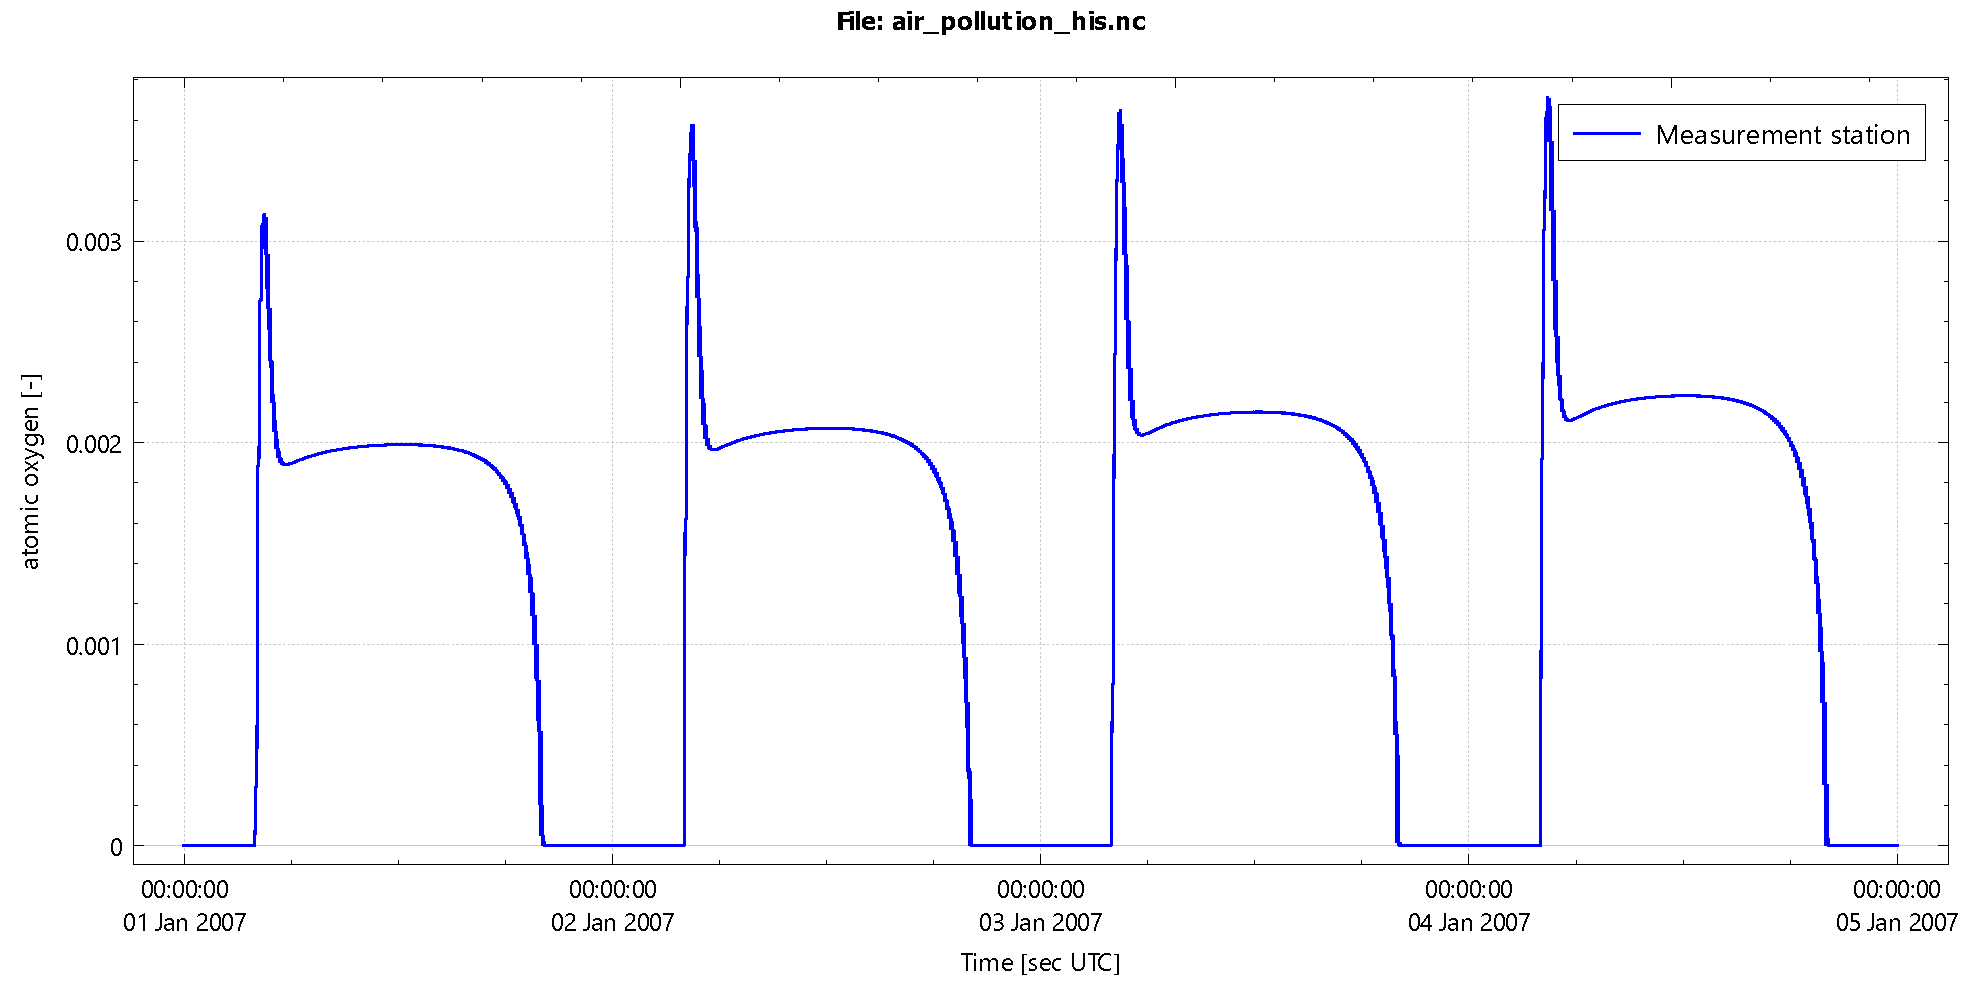
\includegraphics[width=\textwidth]{figures/atomic_oxygon_dt0d5.pdf}
        \caption{Concentration of Atomic Oxygen.}
    \end{subfigure}
    \begin{subfigure}{0.5\textwidth}
        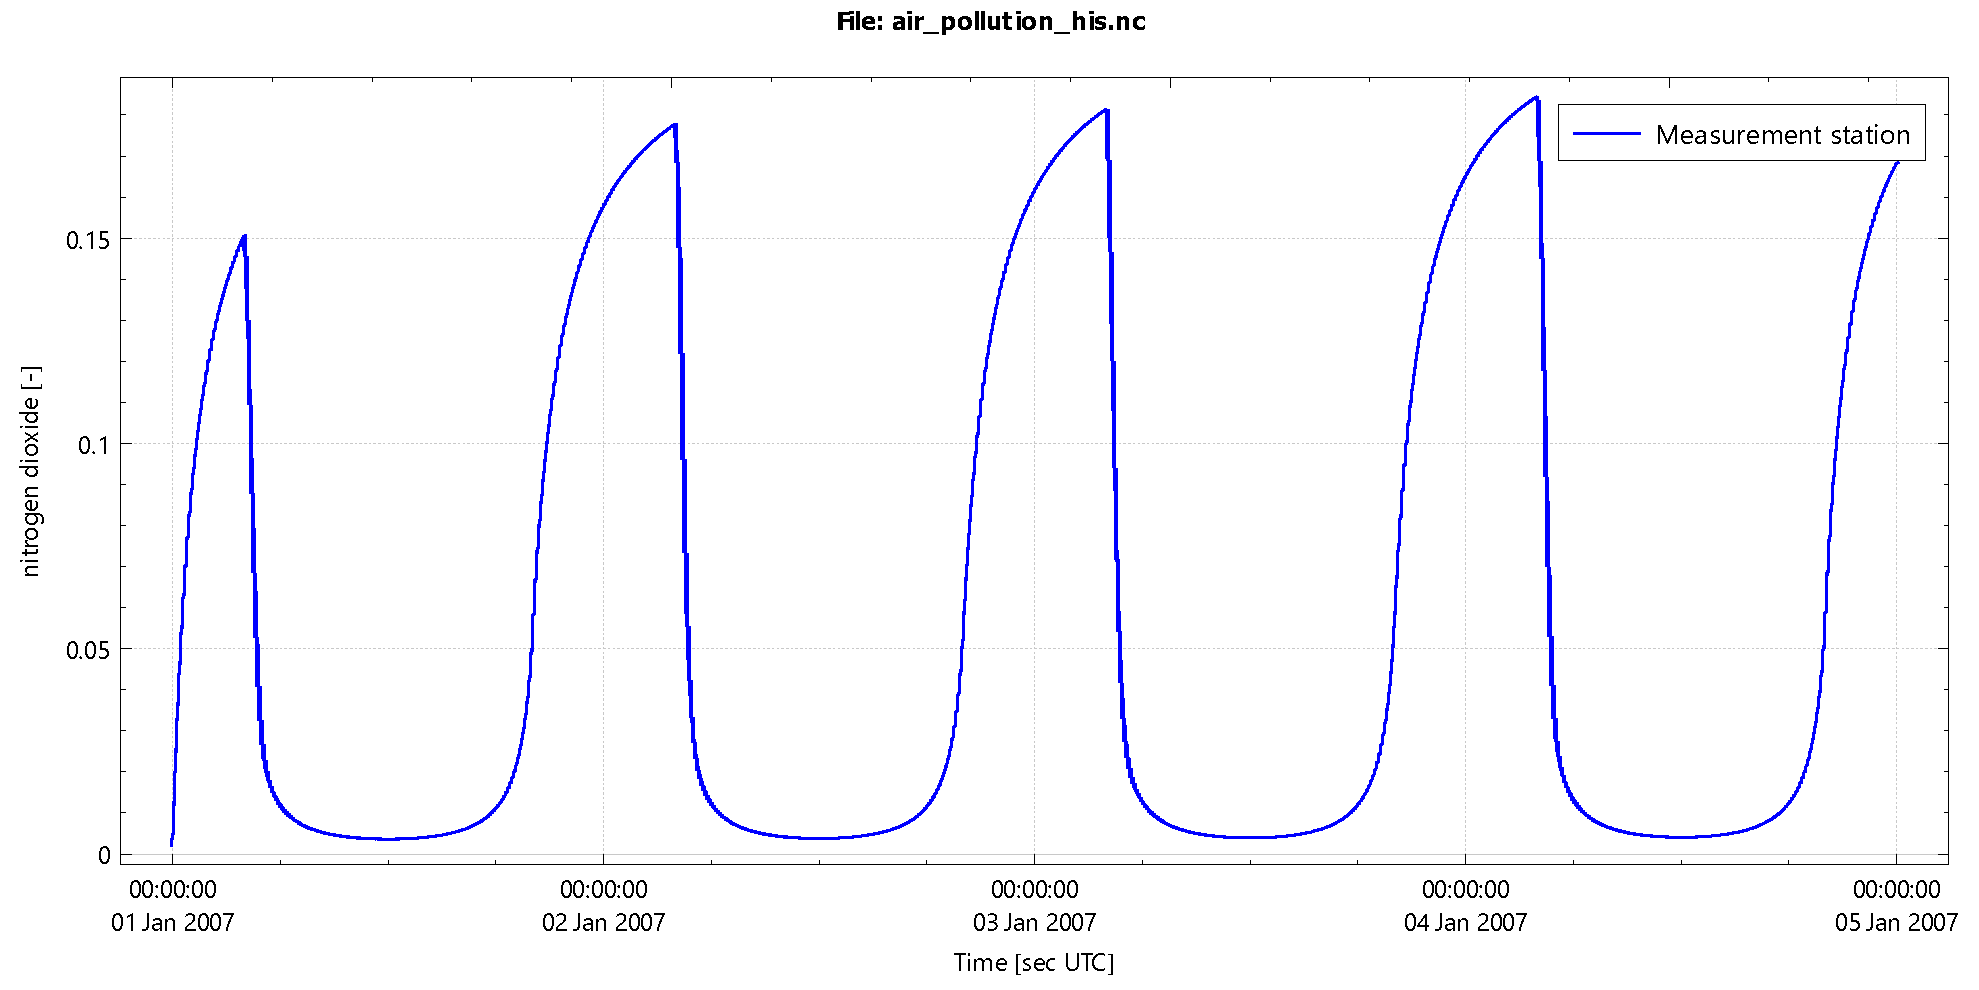
\includegraphics[width=\textwidth]{figures/nitrogen_dioxide_dt0d5.pdf}
        \caption{Concentration of Nitrogen Dioxide.}
    \end{subfigure}
    \begin{subfigure}{0.5\textwidth}
        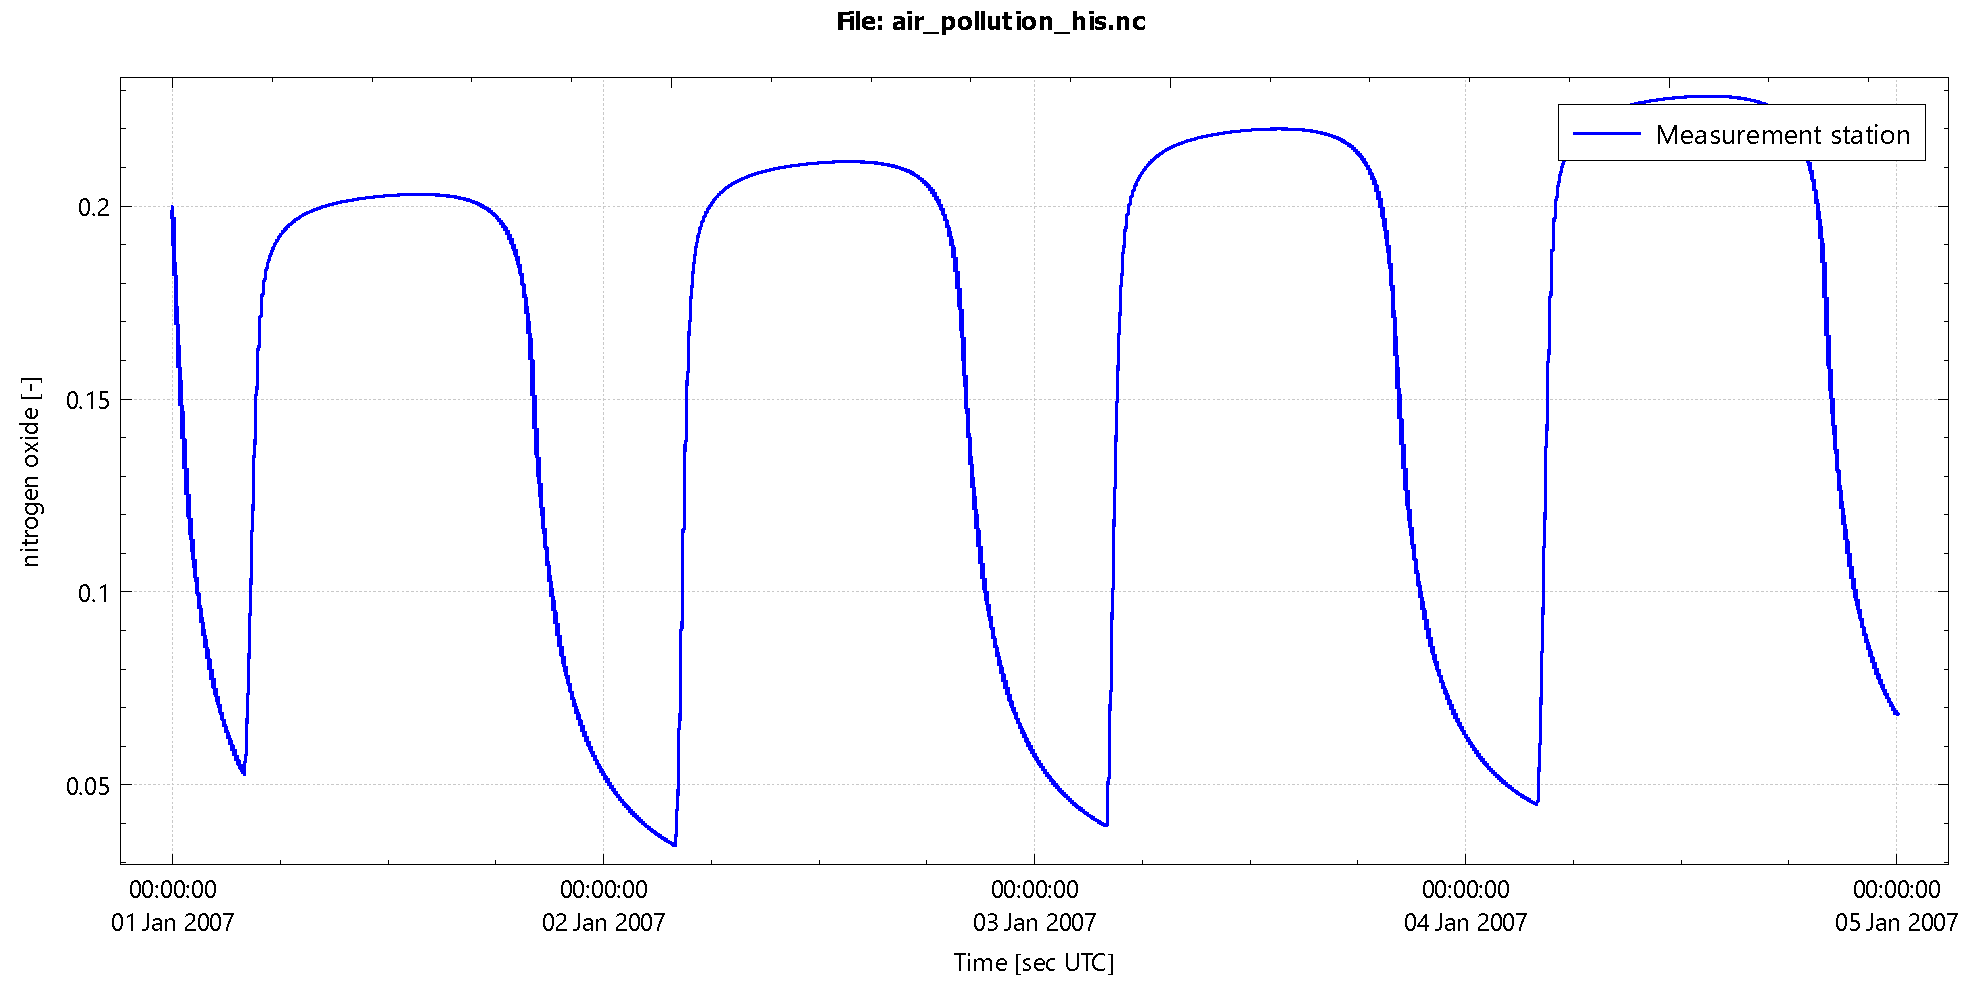
\includegraphics[width=\textwidth]{figures/nitrogen_oxide_dt0d5.pdf}
        \caption{Concentration of Nitrogen Oxide.}
    \end{subfigure}
    \begin{subfigure}{0.5\textwidth}
        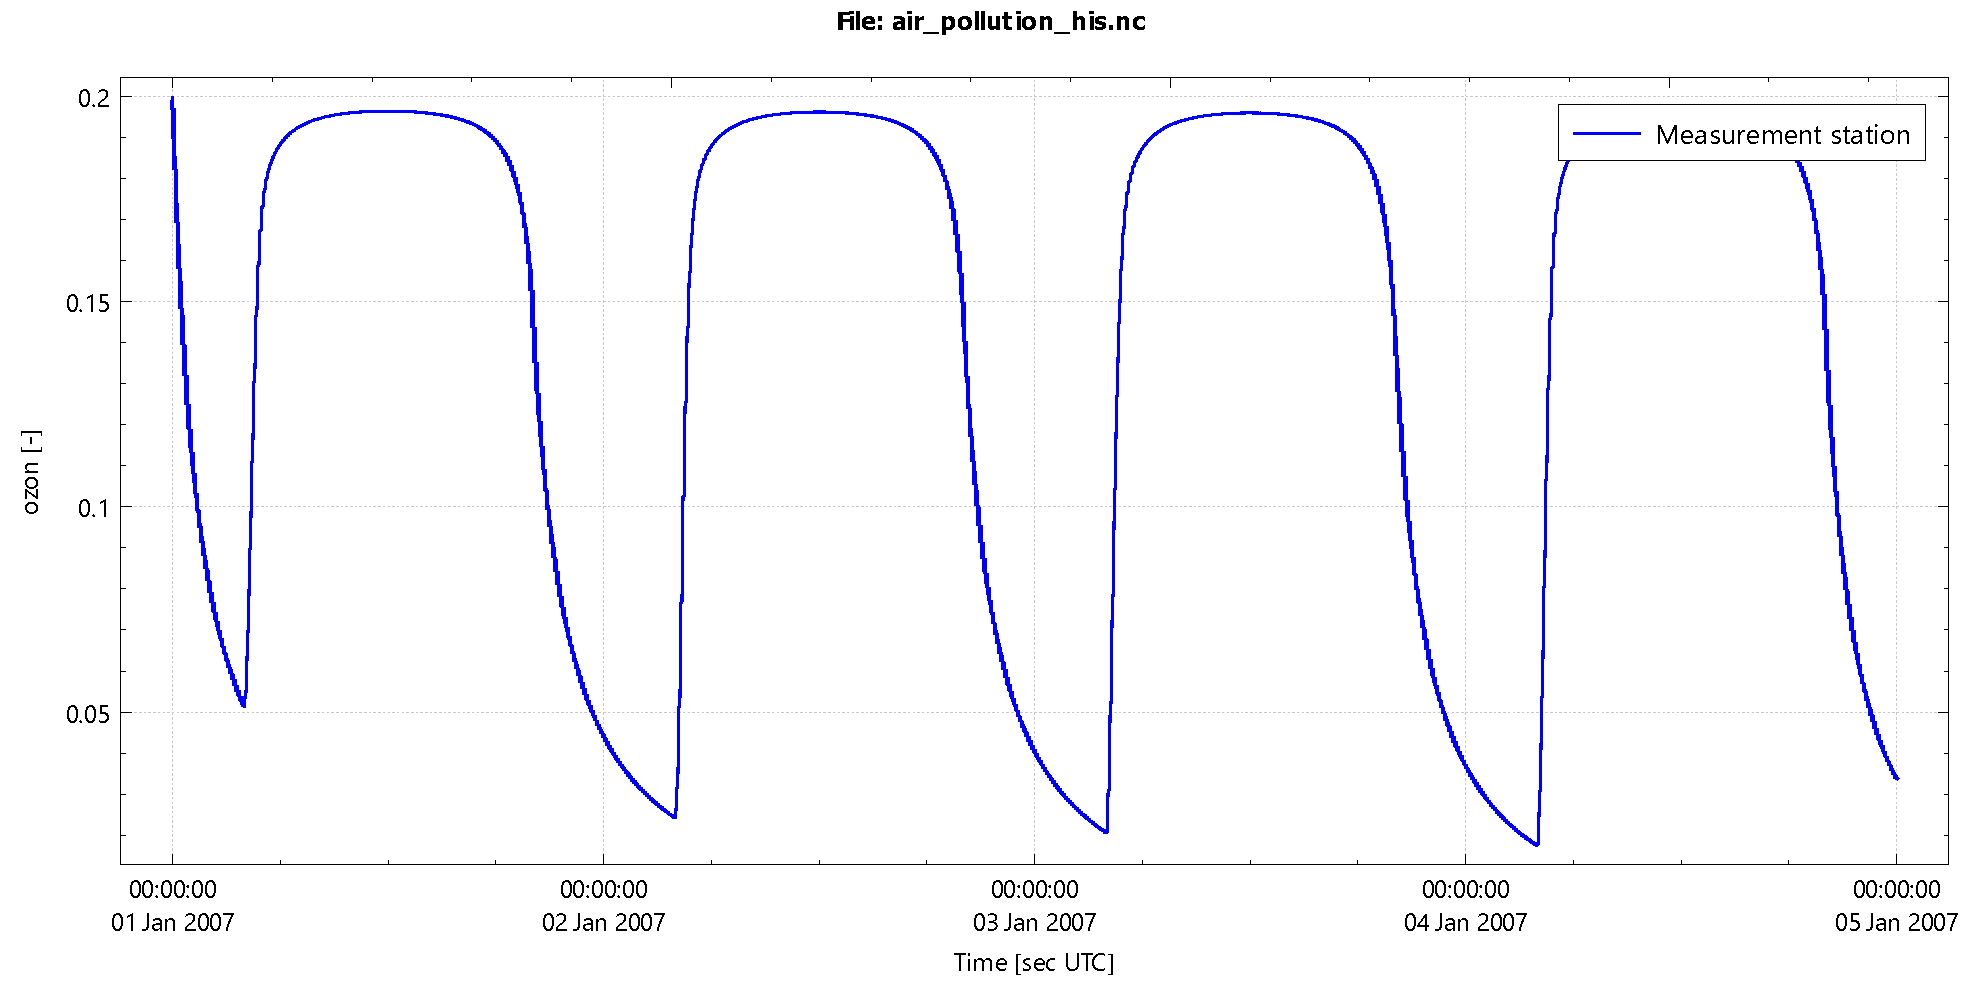
\includegraphics[width=\textwidth]{figures/ozon_dt0d5.pdf}
        \caption{Concentration of Ozon.}
    \end{subfigure}
    \caption{Result plots of the different constituents, compute with a Runge-Kutta 4 time integration with a timestep of \SI{0.5}{[second]}.}
\end{figure}
%------------------------------------------------------------------------------
%\printallbibliography
%\end{document}

%-------------------------------------------------------------------------------
\section{Numerics}
Discretized
\begin{align}
    \frac{1}{\Dt}\Delta u_1^{n+1, p+1} & = - \frac{1}{\Dt}(u_1^{n+1,p} - u_1^n) + k_1 (u_3^{n+\theta,p+1}) - k_2 (u_1^{n+\theta,p+1})
    \\
    \frac{1}{\Dt}\Delta u_2^{n+1, p+1} & = - \frac{1}{\Dt}(u_2^{n+1,p} - u_2^n) + k_1(u_3^{n+\theta,p+1}) - k_3 (u_2^{n+\theta,p+1}) (u_4^{n+\theta,p+1}) +\sigma_2
    \\
    \frac{1}{\Dt}\Delta u_3^{n+1, p+1} & = - \frac{1}{\Dt}(u_3^{n+1,p} - u_3^n) + k_3 (u_2^{n+\theta,p+1}) (u_4^{n+\theta,p+1}) - k_1(u_3^{n+\theta,p+1})
    \\
    \frac{1}{\Dt}\Delta u_4^{n+1, p+1} & = - \frac{1}{\Dt}(u_4^{n+1,p} - u_4^n) + k_2(u_1^{n+\theta,p+1}) - k_3 (u_2^{n+\theta,p+1}) (u_4^{n+\theta,p+1})
\end{align}
Linearization of $\vec{u}^{n+\theta,p+1}$:
\begin{align}
    \frac{1}{\Dt}\Delta u_1^{n+1, p+1} & =
    - \frac{1}{\Dt}(u_1^{n+1,p} - u_1^n) + \\
    & + k_1 (u_3^{n+\theta,p} + \theta \Delta u_3^{n+1, p+1}) - k_2 (u_1^{n+\theta,p} + \theta \Delta u_1^{n+1, p+1})
    \\
    \frac{1}{\Dt}\Delta u_2^{n+1, p+1} & = - \frac{1}{\Dt}(u_2^{n+1,p} - u_2^n) +
    \\
    & + k_1(u_3^{n+\theta,p} + \theta \Delta u_3^{n+1, p+1}) - k_3 (u_2^{n+\theta,p} + \theta \Delta u_2^{n+1, p+1}) (u_4^{n+\theta,p} + \theta \Delta u_4^{n+1, p+1}) +\sigma_2
    \\
    \frac{1}{\Dt}\Delta u_3^{n+1, p+1} & = - \frac{1}{\Dt}(u_3^{n+1,p} - u_3^n) +
    \\
    & +  k_3 (u_2^{n+\theta,p} + \theta \Delta u_2^{n+1, p+1}) (u_4^{n+\theta,p} + \theta \Delta u_4^{n+1, p+1}) - k_1(u_3^{n+\theta,p} + \theta \Delta u_3^{n+1, p+1})
    \\
    \frac{1}{\Dt}\Delta u_4^{n+1, p+1} & = - \frac{1}{\Dt}(u_4^{n+1,p} - u_4^n) +
    \\
    & + k_2(u_1^{n+\theta,p} + \theta \Delta u_1^{n+1, p+1}) - k_3 (u_2^{n+\theta,p} + \theta \Delta u_2^{n+1, p+1}) (u_4^{n+\theta,p} + \theta \Delta u_4^{n+1, p+1})
\end{align}
Rearrange tp $\mat{A}\vec{x}=\vec{b}$
\begin{align}
    \frac{1}{\Dt}\Delta u_1^{n+1, p+1} &  - k_1  \theta \Delta u_3^{n+1, p+1} + k_2  \theta \Delta u_1^{n+1, p+1}  =
    \\
    & = - \frac{1}{\Dt}(u_1^{n+1,p} - u_1^n) + k_1 u_3^{n+\theta,p} - k_2 u_1^{n+\theta,p}
    \\
    \frac{1}{\Dt}\Delta u_2^{n+1, p+1} & - k_1 \theta \Delta u_3^{n+1, p+1}
    + k_3 \theta u_4^{n+1,p} \Delta u_2^{n+1, p+1} + k_3 \theta u_2^{n+1,p} \Delta u_4^{n+1, p+1}  =
    \\
    & = - \frac{1}{\Dt}(u_2^{n+1,p} - u_2^n) + k_1 u_3^{n+\theta,p} - k_3 u_2^{n+\theta,p} u_4^{n+\theta,p} +\sigma_2
    \\
    \frac{1}{\Dt}\Delta u_3^{n+1, p+1} & - k_3 u_2^{n+\theta,p} \theta \Delta u_4^{n+1, p+1} - k_3 u_4^{n+\theta,p} \theta \Delta u_2^{n+1, p+1} + k_1 \theta \Delta u_3^{n+1, p+1}  =
    \\
    & = - \frac{1}{\Dt}(u_3^{n+1,p} - u_3^n) + k_3 u_2^{n+\theta,p} u_4^{n+\theta,p} - k_1 u_3^{n+\theta,p}
    \\
    \frac{1}{\Dt}\Delta u_4^{n+1, p+1}&  - k_2 \theta \Delta u_1^{n+1, p+1}  + k_3 u_2^{n+\theta,p}\theta \Delta u_4^{n+1, p+1} +k_3 u_4^{n+\theta,p} \theta \Delta u_2^{n+1, p+1} =
    \\
    & = - \frac{1}{\Dt}(u_4^{n+1,p} - u_4^n) + k_2 u_1^{n+\theta,p} - k_3 u_2^{n+\theta,p} u_4^{n+\theta,p}
\end{align}


%------------------------------------------------------------------------------
\newpage
\section{Numerical experiment}
%
\begin{longtable}{>{\bfseries}p{6mm-12pt}|p{\textwidth/4-2mm-12pt}|p{\textwidth/4-2mm-12pt}|p{\textwidth/4-2mm-12pt}|p{\textwidth/4-2mm-12pt}}
\caption{Stability of different time integrators for the Air Pollution case.} \\%
\rowcolor{mgreen1}
& \textcolor{white}{\textbf{Time step\newline [s]}}
& \textcolor{white}{\textbf{Euler Explicit}}
& \textcolor{white}{\textbf{Runge-Kutta 4}}
& \textcolor{white}{\textbf{Fully Implicit\newline $\Delta$-formulation}}
\\
\topline
\endfirsthead
\endhead
\endfoot
\bottomline
\endlastfoot
1 & 0.5 & -  & \checkmark & - \\
\midline
2 & 60 & \checkmark  & \checkmark  &  \checkmark \\
\midline
3 & 120 & Unstable & \checkmark &  \checkmark \\
\midline
4 & 180 & - & Unstable & \checkmark \\
\midline
5 & 240 & - & - & \checkmark \\
\midline
6 & 300 & - & - & \checkmark \\
\midline
7 & 900 & - & - & \checkmark \\
\midline
8 & 1800 & - & - & \checkmark \\
\midline
9 & 3600 & - & - & \checkmark \\
\end{longtable}
%

%------------------------------------------------------------------------------
\printallbibliography
\end{document}
